\documentclass[a4paper,7pt]{jsarticle}
\usepackage{url}
\usepackage[dvipdfmx]{graphicx}
\usepackage{epsfig}
\usepackage{amsmath}
\usepackage{amssymb}
\usepackage{times}
\usepackage{ascmac}
\usepackage{here}
\usepackage{txfonts}
\usepackage{listings, jlisting}

\renewcommand{\lstlistingname}{リスト}
\lstset{%language=perl,
  basicstyle=\ttfamily\scriptsize,
  commentstyle=\textit,
  classoffset=1,
  keywordstyle=\bfseries,
  frame=tRBl,
  framesep=5pt,
  showstringspaces=false,
  numbers=left,
  stepnumber=1,
  numberstyle=\tiny,
  tabsize=2,
  morekeywords={set, script, on, of, item, property, tell, as,
  from, to, is, equal, end, if, else, then, try, error, rest,
  application, every, whose, repeat, with, in, first}
}



\title{ソフトウェアサイエンスセミナー 資料 \\{\large{AppleScript概説}}}
\author{青木大祐}

\begin{document}
\maketitle
\section{AppleScriptとは}
1993年にAppleが開発したSystem 7向けプログラミング言語である。以降のMac
OSにはすべて実行環境が付属しており、動作させることができる。

プログラミングパラダイムとしてはイベントドリブンのオブジェクト指向を採用
している。これは通常のプログラミング言語とは多少目的が異なり、「Mac OSに
おけるいろいろな操作を自動化する」ことに主眼が置かれているためである。例
えば「フォルダアクション」というイベントに、用意したAppleScriptを関連付
けることで、あるフォルダ内に変更が加えられた時の処理を記述することが出来
る。\\

また、大きな特徴の一つとして「利用者として一般的な(非技術者の)Macユーザ
をも想定している」という側面がある。そのため、AppleScriptの文法は非常に
英語に近い記述が可能であり、またそれを可能にするため様々な工夫が取り入れ
られている。リリース当初は英語だけでなく、日本語を含む様々な言語での記述
が可能であったが、現行のMac OSXでは英語のもののみが採用されている。

\section{文法}
\subsection{変数}
変数への値の設定はset文を使って行う。なお、ハイフン2つ以降の文字列はすべ
てコメントとして無視される。
\begin{lstlisting}
 set a to 1 -- integer
 set b to "abc" -- string
 set c to {1, 3, 5} -- list
 set d to {a:1, b:3, c:5} -- record
\end{lstlisting}
変数には型がないため、どんなデータでも格納することが出来る。データ型のキャ
ストはasを使う。
\begin{lstlisting}
 set a to 1 as string
\end{lstlisting}
リストにも型の制約はないので、どのような型のデータでも混在させることが出
来る。レコード型についても同様。
\subsection{リスト}
リストの要素へのアクセスは以下のように行う。
\begin{lstlisting}
 set listvar to {1,2,3}

 --リストの先頭要素を取得
 item 1 of listvar
 first item of listvar
 listvar's first item

 --リストの先頭に要素を追加
 set beginning of listvar to 1

 --リストの末尾に要素を追加
 set end of listvar to 1

 --リストの結合
 set listvar to listvar & anotherlist
\end{lstlisting}

\subsection{関数(イベントハンドラ)}
AppleScriptに関数というものは無く、イベントハンドラを定義した上でイベン
トを明示的に発生させることでこれを実現する。\\

イベントハンドラの定義は以下のように記述する。
\begin{lstlisting}
 on myEvent(arg)
  -- 適当に処理を書く
 end myEvent
\end{lstlisting}
イベントを発生させるには、いわゆる関数呼び出しのように記述すれば良い。
\begin{lstlisting}
 myEvent(arg)
\end{lstlisting}
また、「英語っぽさ」を高めるために定義済みラベルを用いた引数の定義ができる。
\begin{lstlisting}
 on getElements from startIndex to endIndex
  -- 要素を取ってくる
 end getElements

 --呼び出し
 getElements from 1 to 10 
\end{lstlisting}
定義済みラベルとして「out, above, against, apart from, around, aside
from, at, below, beneath, beside, between, by, for, from, instead of,
into, on, onto, out of, over, since, thru (or through), under」を自由に
記述することができる。\\
\newpage
以下に、リストに含まれる数値の合計を求めるスクリプトを示す。リストの中に
リストが含まれている場合は、そのリスト内の合計値をリストの数値とする。

\begin{lstlisting}
on run
	sum({1, 2, 3, {1, 2}})
end run

on sum(arg)
	-- 数値リストの総和を求める
	-- リストが含まれている場合は再帰的に中身も合計する
	if arg is equal to {} then
		set result to 0
	else if class of arg's first item is equal to list then
		-- 先頭の要素がリストなら、そちらにもsumを適用
		set result to sum(arg's first item) + sum(arg's rest)
	else
		try
			set result to (arg's first item as number) + sum(arg's rest)
		on error
			--数値に変換できない要素は無視
			set result to sum(arg's rest)
		end try
	end if
end sum
\end{lstlisting}
ほとんど英語として読み下すことができるようなソースコードになっている。


\subsection{scriptオブジェクト}
scriptオブジェクトは、いわゆるオブジェクト指向言語におけるオブジェクトで
ある。AppleScriptにはクラスという概念は無く、プロトタイプベースのオブジェ
クト指向であると言える。

scriptオブジェクトはプロパティ(property)とイベントハンドラを持つことが出
来る。

\begin{lstlisting}
script myObj
	property myInt : 0
	property myStr : "hoge"
	
	on myEvent(arg)
		-- do someting
	end myEvent
end script
\end{lstlisting}
また、parentを指定することでオブジェクトを継承することが出来る。
JavaScriptと同じようにプロトタイプチェーンを構成することで、そのscriptオ
ブジェクトに無いpropertyを祖先に向かって探していく。

\begin{lstlisting}
script myObjExtended
	property parent : myObj
 --etc...
end script
\end{lstlisting}

scriptオブジェクトのハンドラを呼び出すにはtell文を使ってイベントを通知す
る。

\begin{lstlisting}
tell myObjExtended to myEvent(1)
\end{lstlisting}
また、tellブロックを使うことで、その中でのイベント通知先を暗黙的に指定す
ることが出来る。
\begin{lstlisting}
tell myObj
	log myEvent(1) --暗黙的にmyObjがレシーバだと見なされる
	log myInt of myObj --省略できるのはハンドラだけ
end tell
\end{lstlisting}

\newpage

\subsection{Applicationオブジェクト}
AppleScriptでは、Mac OSのOSA(Open Scripting Architecture)という機能を経由
して、ほかのOSXアプリケーションに対してApple Eventを通知することが出来る。
OSXプリインストールのアプリケーション群には多くのイベントが用意されてお
り、これを活用することで、より快適なコンピューティング生活を送ることが出来る
だろう。

\begin{center}
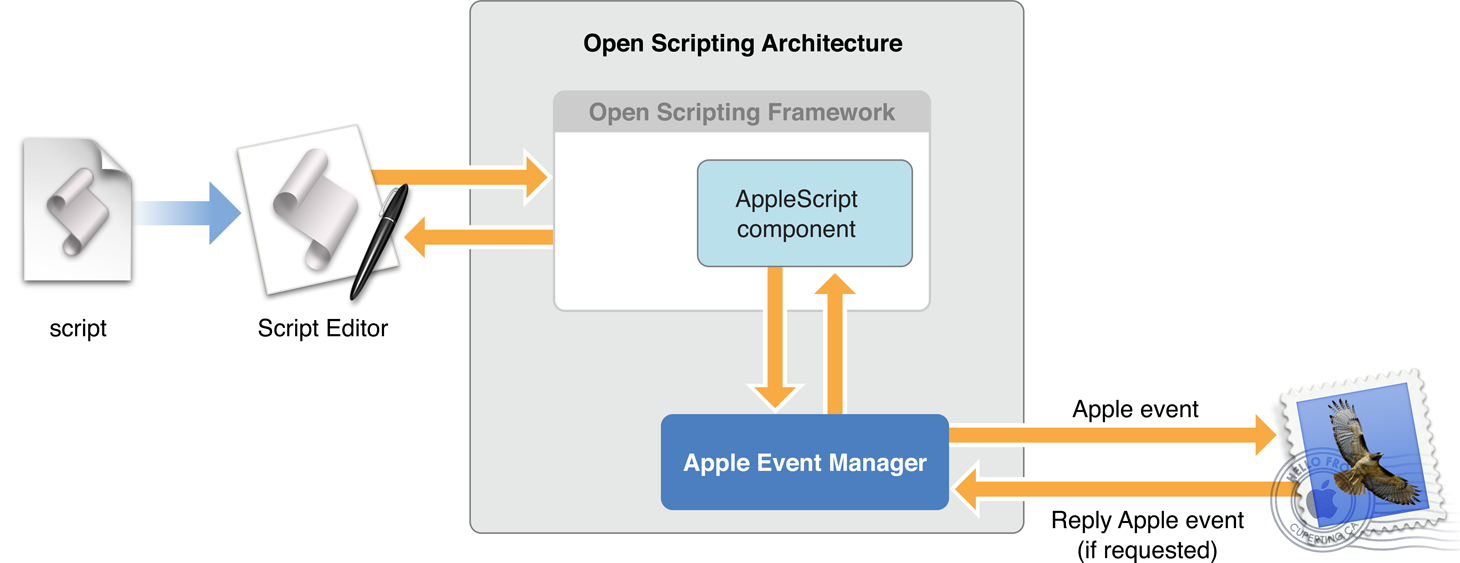
\includegraphics[width=10cm]{osa.png}\\ 
\end{center}

また、System Eventというイベントが用意されており、キーボードやマウスなど
の操作をエミュレートすることが出来る。例えサードパーティ製の「行儀の悪い」
アプリケーションであっても、System Eventを駆使することで強引に自動化する
ことが可能である。\\

以下に、FinderとiTunesのApplicationオブジェクトにイベントを通知して、指定したディレクトリ以下のM4A音楽ファ
イルをすべてライブラリに追加するスクリプトを示す。

\begin{lstlisting}
set src to choose folder
set target_files to getFiles(src)
tell application "iTunes"
	repeat with f in target_files
		try
			add f
			delay 1
		on error
			log f
		end try
	end repeat
end tell

on getFiles(target_folder)
	tell application "Finder"
		tell folder target_folder
			set tmp to {}
			log "called"
			set m4a_files to (get every file of target_folder whose file type is "M4A ")
			repeat with f1 in m4a_files
				set end of tmp to f1 as alias
			end repeat
			
			set f_list to (get every folder of target_folder)
			repeat with f2 in f_list
				set ans to getFiles(f2) of me
				if (count of ans) is not 0 then
					set tmp to tmp & ans
				end if
			end repeat
			
			set result to tmp
			
		end tell
	end tell
end getFiles
\end{lstlisting}
\end{document}

